\documentclass[titlepage, a4paper]{article}
\usepackage[english]{babel}
\usepackage[utf8]{inputenc}
\usepackage{graphicx}
\usepackage{color}
\usepackage{mathtools}
\usepackage{float}
\usepackage[parfill]{parskip}
\usepackage[margin=10pt,font=small,labelfont=bf,labelsep=endash]{caption}
\usepackage{epstopdf}
\usepackage{listings}
\epstopdfsetup{suffix=}
\DeclareGraphicsExtensions{.ps}
\DeclareGraphicsRule{.ps}{pdf}{.pdf}{`ps2pdf -dEPSCrop -dNOSAFER #1 \noexpand\OutputFile}

\lstset{literate=%
    {å}{{\r{a}}}1
    {ä}{{\"a}}1
    {ö}{{\"o}}1
    {Å}{{\r{A}}}1
    {Ä}{{\"A}}1
    {Ö}{{\"O}}1
}

\newcommand{\todo}[1] {\textbf{\textcolor{red}{#1}}}

\usepackage{fancyhdr}
\fancyhead[L]{}
\pagestyle{fancy}
\rhead{Alexander Yngve \\ Pål Kastman}
\chead{TDDC78}
\thispagestyle{empty}

\begin{document}

{\ }\vspace{45mm}

\begin{center}
  \Huge \textbf{TDDC78: Lab Report}
\end{center}
\begin{center}
  \Large Lab 2: Pthreads
\end{center}

\vspace{250pt}

\begin{center}
  \begin{tabular}{|*{3}{p{40mm}|}}
    \hline
    \textbf{Name} & \textbf{PIN} & \textbf{Email} \\ \hline
           {Alexander Yngve} & {930320-6651} & {aleyn573@student.liu.se} \\ \hline
           {Pål Kastman} & {851212-7575} & {palka285@student.liu.se} \\ \hline
  \end{tabular}
\end{center}
\newpage

\tableofcontents
\thispagestyle{empty}
\newpage

\section{Introduction}
This lab consists just as the previous lab 1 of two image filters: blur filter and threshold filter.

The difference from the first lab where we used MPI is that we will instead use Pthreads in this lab. All the threads will have access to the same data so that we won't have to distribute this to the new threads.


\subsection{Blur filter}
The blur filter uses a normal distribution together with a given radius to calculate the mean value for every pixel in an image, this will create a blur the given image.


\subsection{Threshold filter}
The threshold filter first calculates a mean value for every pixel in the image, it will then go through the image one more time and either set every pixel to black or white depending if the pixel value is over or under the calculated mean value.

\section{Our implementation}
This section will describe how we used MPI to parallelize the execution of the programs.

\subsection{Blur filter}
Just as in the first lab, each thread will have an overlapping region of the image that they will apply the filter to. But in this lab the threads will have access to the same data.

To give the threads this data we define a struct called thread\_data which contains pointer to all the necessary data, which is calculated by the first thread before it starts the other threads. It also contains pointer to the image and an intermediary image.

When we create the threads we pass in the struct along with the function thread\_blur\_x, this will run the filter in the x axis, and update the intermediary image. The main thread will wait for all the threads by running pthreads\_join. When all the threads are done, the main thread will then create new threads but instead pass in the thread\_blur\_y function which will run the filter in the y axis.

The reason we do it this way is that the threads are now working on the same memory and if we run the filter as it is, then one thread might read a value that another thread have changed. This is not good, and we want to avoid it.

The main thread will then save the result and exit.

\subsection{Threshold filter}
Here we define a struct just as in the blur filter, we assign areas to the new threads and start them. The threads will run the function threshold\_average, this function will calculate the average values of their area and save this to the struct.

When all the tasks are done, the main task will calculate a total average value from the various average values in the structs. Then it will save this value in all the structs and start new threads, passing in the threshold\_filter function to the threads, and now they will run the filter.

When done the main thread, which have waited for the other threads, will save the result and exit.

\section{Execution times}
In this section we will present the execution times of the filters.

It is worth mentioning that the times for all graphs below are in seconds.

The tests were performed on four images with sizes as can be seen in \ref{tab:table1}.

\begin{table}[H]
  \centering
  \caption{The sizes for the images used in the tests.}
  \begin{tabular}{|*{3}{p{30mm}|}}
    \hline
    \textbf{Image name} & \textbf{x pixels } & \textbf{y pixels} \\ \hline
           {im1.ppm} & {676} & {763} \\ \hline
           {im2.ppm} & {1024} & {1024} \\ \hline
           {im3.ppm} & {1600} & {1200} \\ \hline
           {im4.ppm} & {3000} & {3000} \\ \hline
  \end{tabular}
  \label{tab:table1}
\end{table}

We accidentally made the graphs for lab1 from the results of image 1 and image 2, and the graphs for lab 2 from the results of image 3 and image 4 and hence, the reader can't compare the difference in execution times between pthreads and MPI. This wasn't not intentionally done.

\subsection{Blur filter}
Our result show that if we increase the number of threads, we will get a decrease in time. But this relationship is not linear due to deminishing returns, since the problem is not perfectly parallell the serial section sections start to dominate the execution time.

The results for image 3 and image 4 can the seen in figure \ref{fig:im3-blur} and figure \ref{fig:im4-blur} respectively. 

\begin{figure}[H]
  \centering
  \scalebox{0.48}{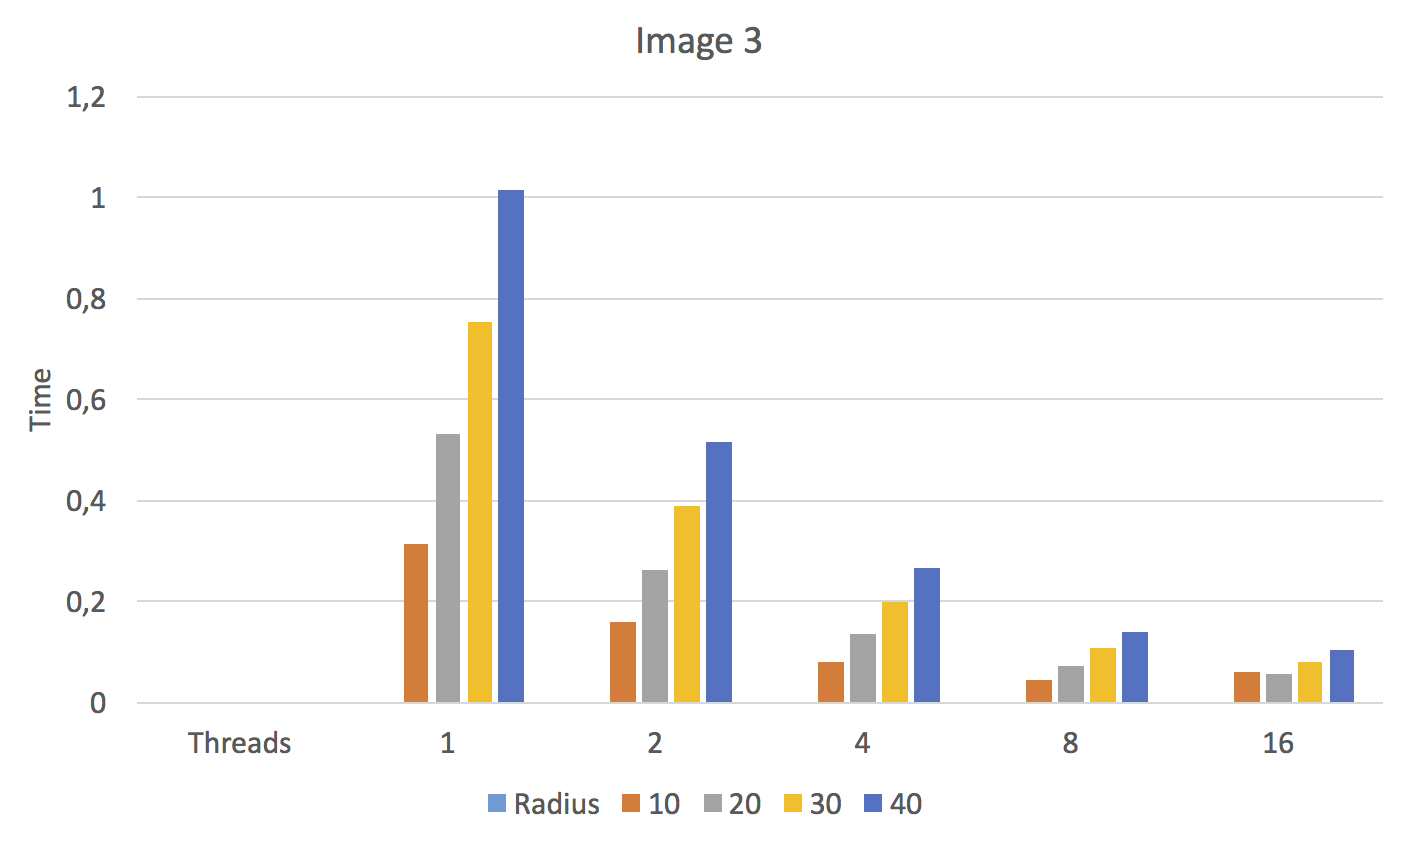
\includegraphics{img/im3-blur.png}}
  \caption{Result for the blur filter run on image 3.}
  \label{fig:im3-blur}
\end{figure}

\begin{figure}[H]
  \centering
  \scalebox{0.48}{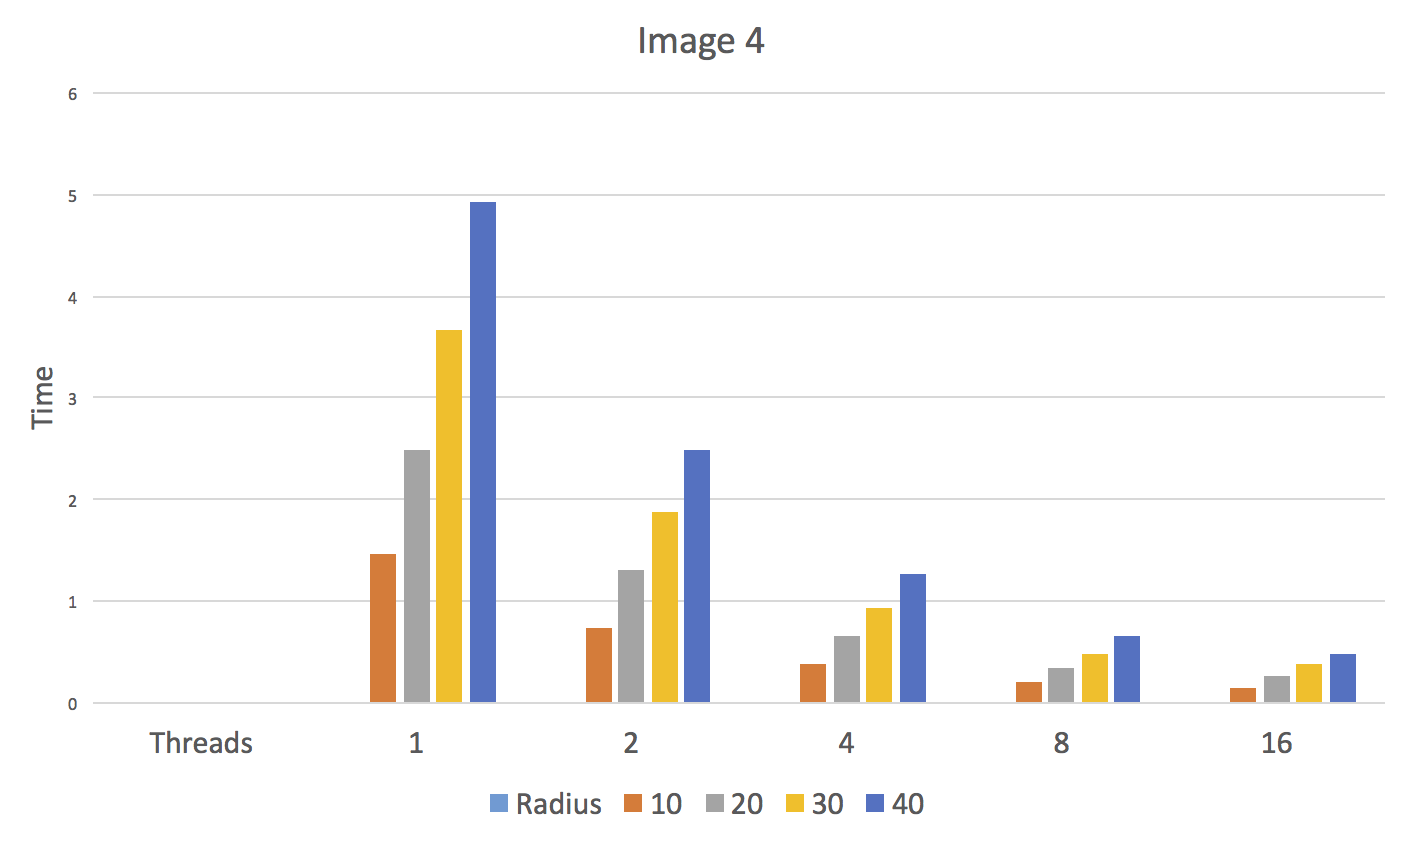
\includegraphics{img/im4-blur.png}}
  \caption{Result for the blur filter run on image 4.}
  \label{fig:im4-blur}
\end{figure}


\subsection{Threshold filter}
We obtained the same pattern of results for this filter as for the blur filter. Executions times for all images can be seen in figure \ref{fig:threshold}

\begin{figure}[H]
  \centering
  \scalebox{0.48}{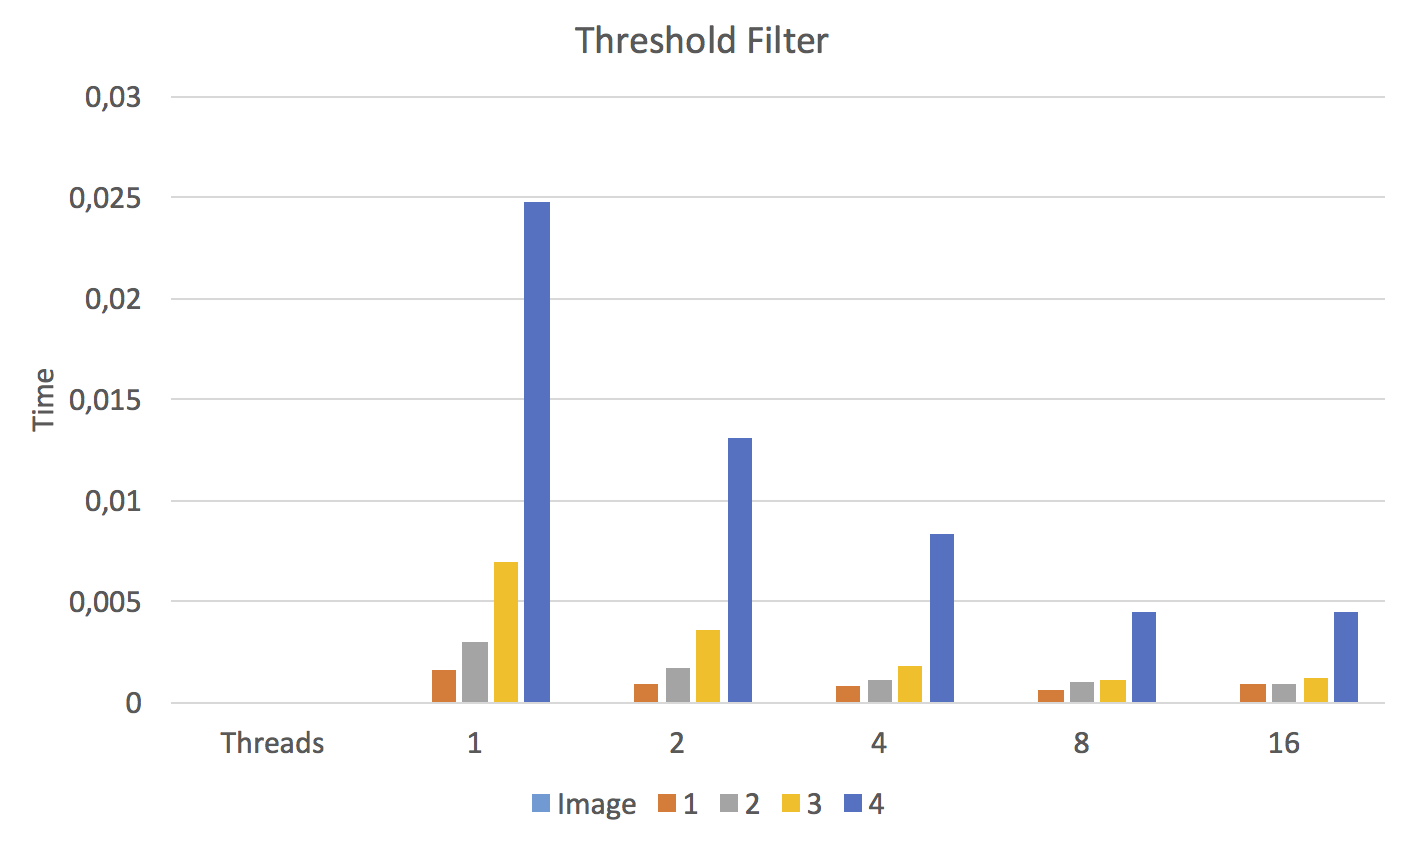
\includegraphics{img/threshold.png}}
  \caption{Result for the threshold filter.}
  \label{fig:threshold}
\end{figure}


\end{document}

%% \begin{table}[H]
%%   \centering
%%   \caption{Miss rates}
%%   \begin{tabular}{|*{3}{p{20mm}|}}
%%     \hline
%%     \textbf{Miss rates} & {test1} & {test2} \\ \hline
%%            {cache1} & {0.0091} & {0.1577} \\ \hline
%%            {cache2} & {0.0177} & {0.0235} \\ \hline
%%   \end{tabular}
%%   \label{tab:table1}
%% \end{table}


%% \begin{figure}[H]
%% 	\centering
%% 	\scalebox{0.342}{\includegraphics{img/data-cache.png}}
%% 	\caption{Only data stored in cache.}
%% 	\label{fig:data-cache}
%% \end{figure}
